\newpage
\section{Control System Design}

In this section the autopilot will be developed. The autopilot uses the desired course angle, $\psi_r$ as reference. For the MatLab simulations in this project, $\psi_r = 30^\circ$, as the linearized model only holds for small deviations in $\psi$. 


%%%%%%%%%%%%%%%%%%%%%%%%%%%%%%%%%%%%%%%%%
% PD Controller Design
%%%%%%%%%%%%%%%%%%%%%%%%%%%%%%%%%%%%%%%%%
\subsection{PD Controller Design}

From earlier we had the following equation, which the PD controller is based on:

\begin{equation*}
    H(s) = \frac{{\psi (s)}}{{\delta (s)}} = \frac{K}{{s(Ts + 1)}}
\end{equation*}

This provides the following transfer function for our PD controller:

\begin{equation}
    H_{pd}(s) = K_{pd}\frac{1+T_{d}s}{1+T_{f}s}
\end{equation}

$T_{d}$ is chosen such that the time constant term from the ship transfer function is cancelled, $T_{d} = T$, and we obtain the open-loop transfer function:

\begin{equation}
    H(s) = H_{pd}H_{ship}\frac{K K_{pd}}{T_{f}s^2+s}
\end{equation}

Phase margin and cut-off frequency are respectively chosen to be $\phi = 50^\circ$ and $\omega_{c} = 0.1 rad/s$. These parameters will help us find $K_{pd}$ and $T_{f}$, thus the relationship betweeen cut-off frequency and phase margin are:

\begin{equation}\label{phi}
    \phi  = {180^o} + \angle H(j\omega c)
\end{equation}

\begin{equation}\label{relat}
    1 = H(j\omega c)H( - j\omega c)
\end{equation}

(\ref{phi}) and (\ref{relat}) provide following results for $K_{pd}$ and $T_{f}$:

\begin{equation*}
    {T_f} = \frac{1}{{\tan \phi {\omega _c}}} = 8.391
\end{equation*}

\begin{equation*}
    {K_{pd}} = \sqrt {\frac{{{T_f}^2{\omega _c}^4 + {\omega _c}^2}}{{{K^2}}}}  = 0.7493
\end{equation*}

The Bode diagram in Figure \ref{plot:3a} shows the results obtained.
%%%% FIGURE %%%%%

\begin{figure}[!htb]
    \caption{Bode diagram}
    \centering
    \centerline{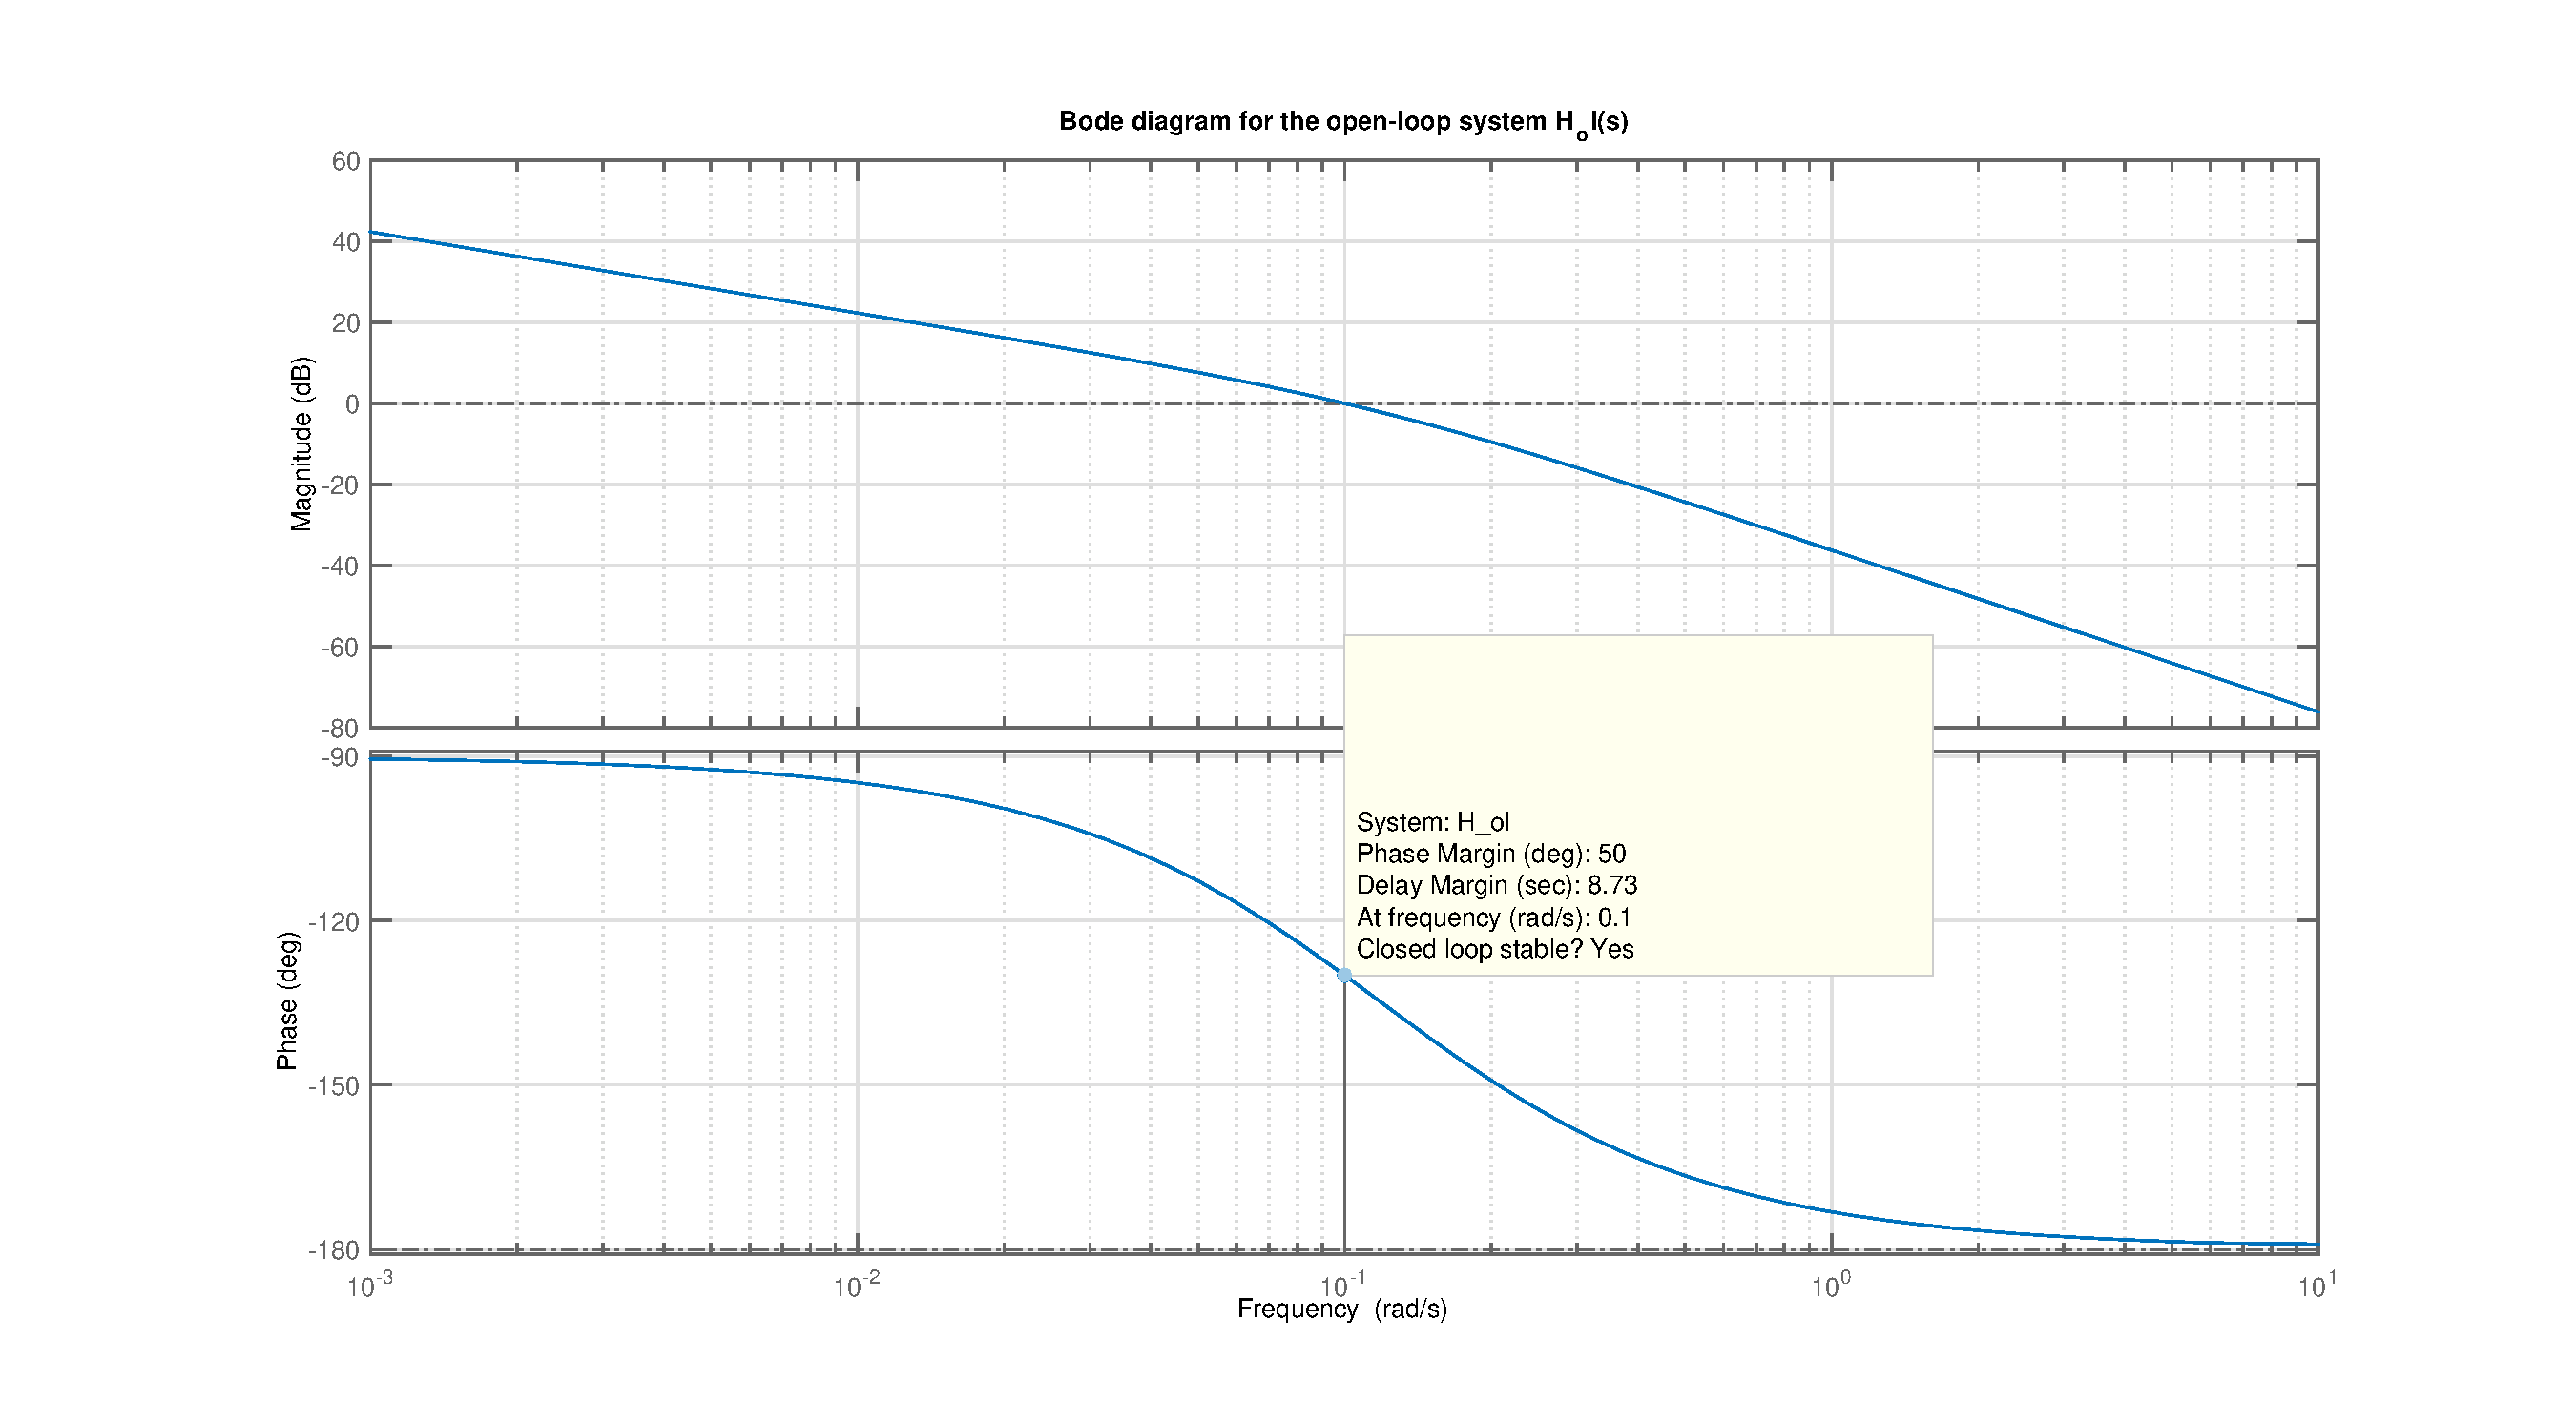
\includegraphics[scale=0.35]{plots/3a}} %This graph is simply too big, i'll fix later.
\label{plot:3a}
\end{figure}

\newpage
%%%%%%%%%%%%%%%%%%%%%%%%%%%%%%%%%%%%%%%%%
% Simulating without disturbances
%%%%%%%%%%%%%%%%%%%%%%%%%%%%%%%%%%%%%%%%%
\subsection{Simulating without disturbances}

In figure \ref{plot:3b} the system simulated without any form of disturbance is displayed. The system is overdamped, but hence its fast convergence to the reference it is only slightly overdamped. The plot of the rudder angle ($\delta$) shows that the actuation is noisy, caused by measurement noise. This might cause undesirable wear on the rudder. 

%%% FIGURE %%%%
\begin{figure}[!htb]
    \caption{Autopilot without disturbances}
    \centering
    \centerline{\includegraphics[scale=0.8]{plots/3b}} %This graph is simply too big, i'll fix later.
    \label{plot:3b}
\end{figure}

\newpage
%%%%%%%%%%%%%%%%%%%%%%%%%%%%%%%%%%%%%%%%%
% Simulating with current disturbance
%%%%%%%%%%%%%%%%%%%%%%%%%%%%%%%%%%%%%%%%%
\subsection{Simulating with current disturbance}

This system is simulated with a current disturbance, displayed in figure \ref{plot:3c}. In the model, the effect of the current is a rudder angle bias ($b$). The rudder angle bias ($b$) gives the system a steady-state error, since there is no feed forward or integral action in the controller.

%%%%% FIGURE %%%%%%
\begin{figure}[!htb]
    \caption{Autopilot with current disturbances}
    \centering
    \centerline{\includegraphics[scale=0.8]{plots/3c}} %This graph is simply too big, i'll fix later.
\label{plot:3c}
\end{figure}

\newpage
%%%%%%%%%%%%%%%%%%%%%%%%%%%%%%%%%%%%%%%%%
% Simulating with wave disturbance
%%%%%%%%%%%%%%%%%%%%%%%%%%%%%%%%%%%%%%%%%
\subsection{Simulating with wave disturbance}

In figure \ref{plot:3d} the system simulated with wave disturbance is displayed. The waves cause a disturbance on the yaw angle ($\psi_{\omega}$). This disturbance is of high frequency with relative high amplitude, which makes the actuation of the rudder noisy. 

%%%% FIGURE %%%%%%%

\begin{figure}[!htb]
    \caption{Autopilot with wave disturbances}
    \centering
    \centerline{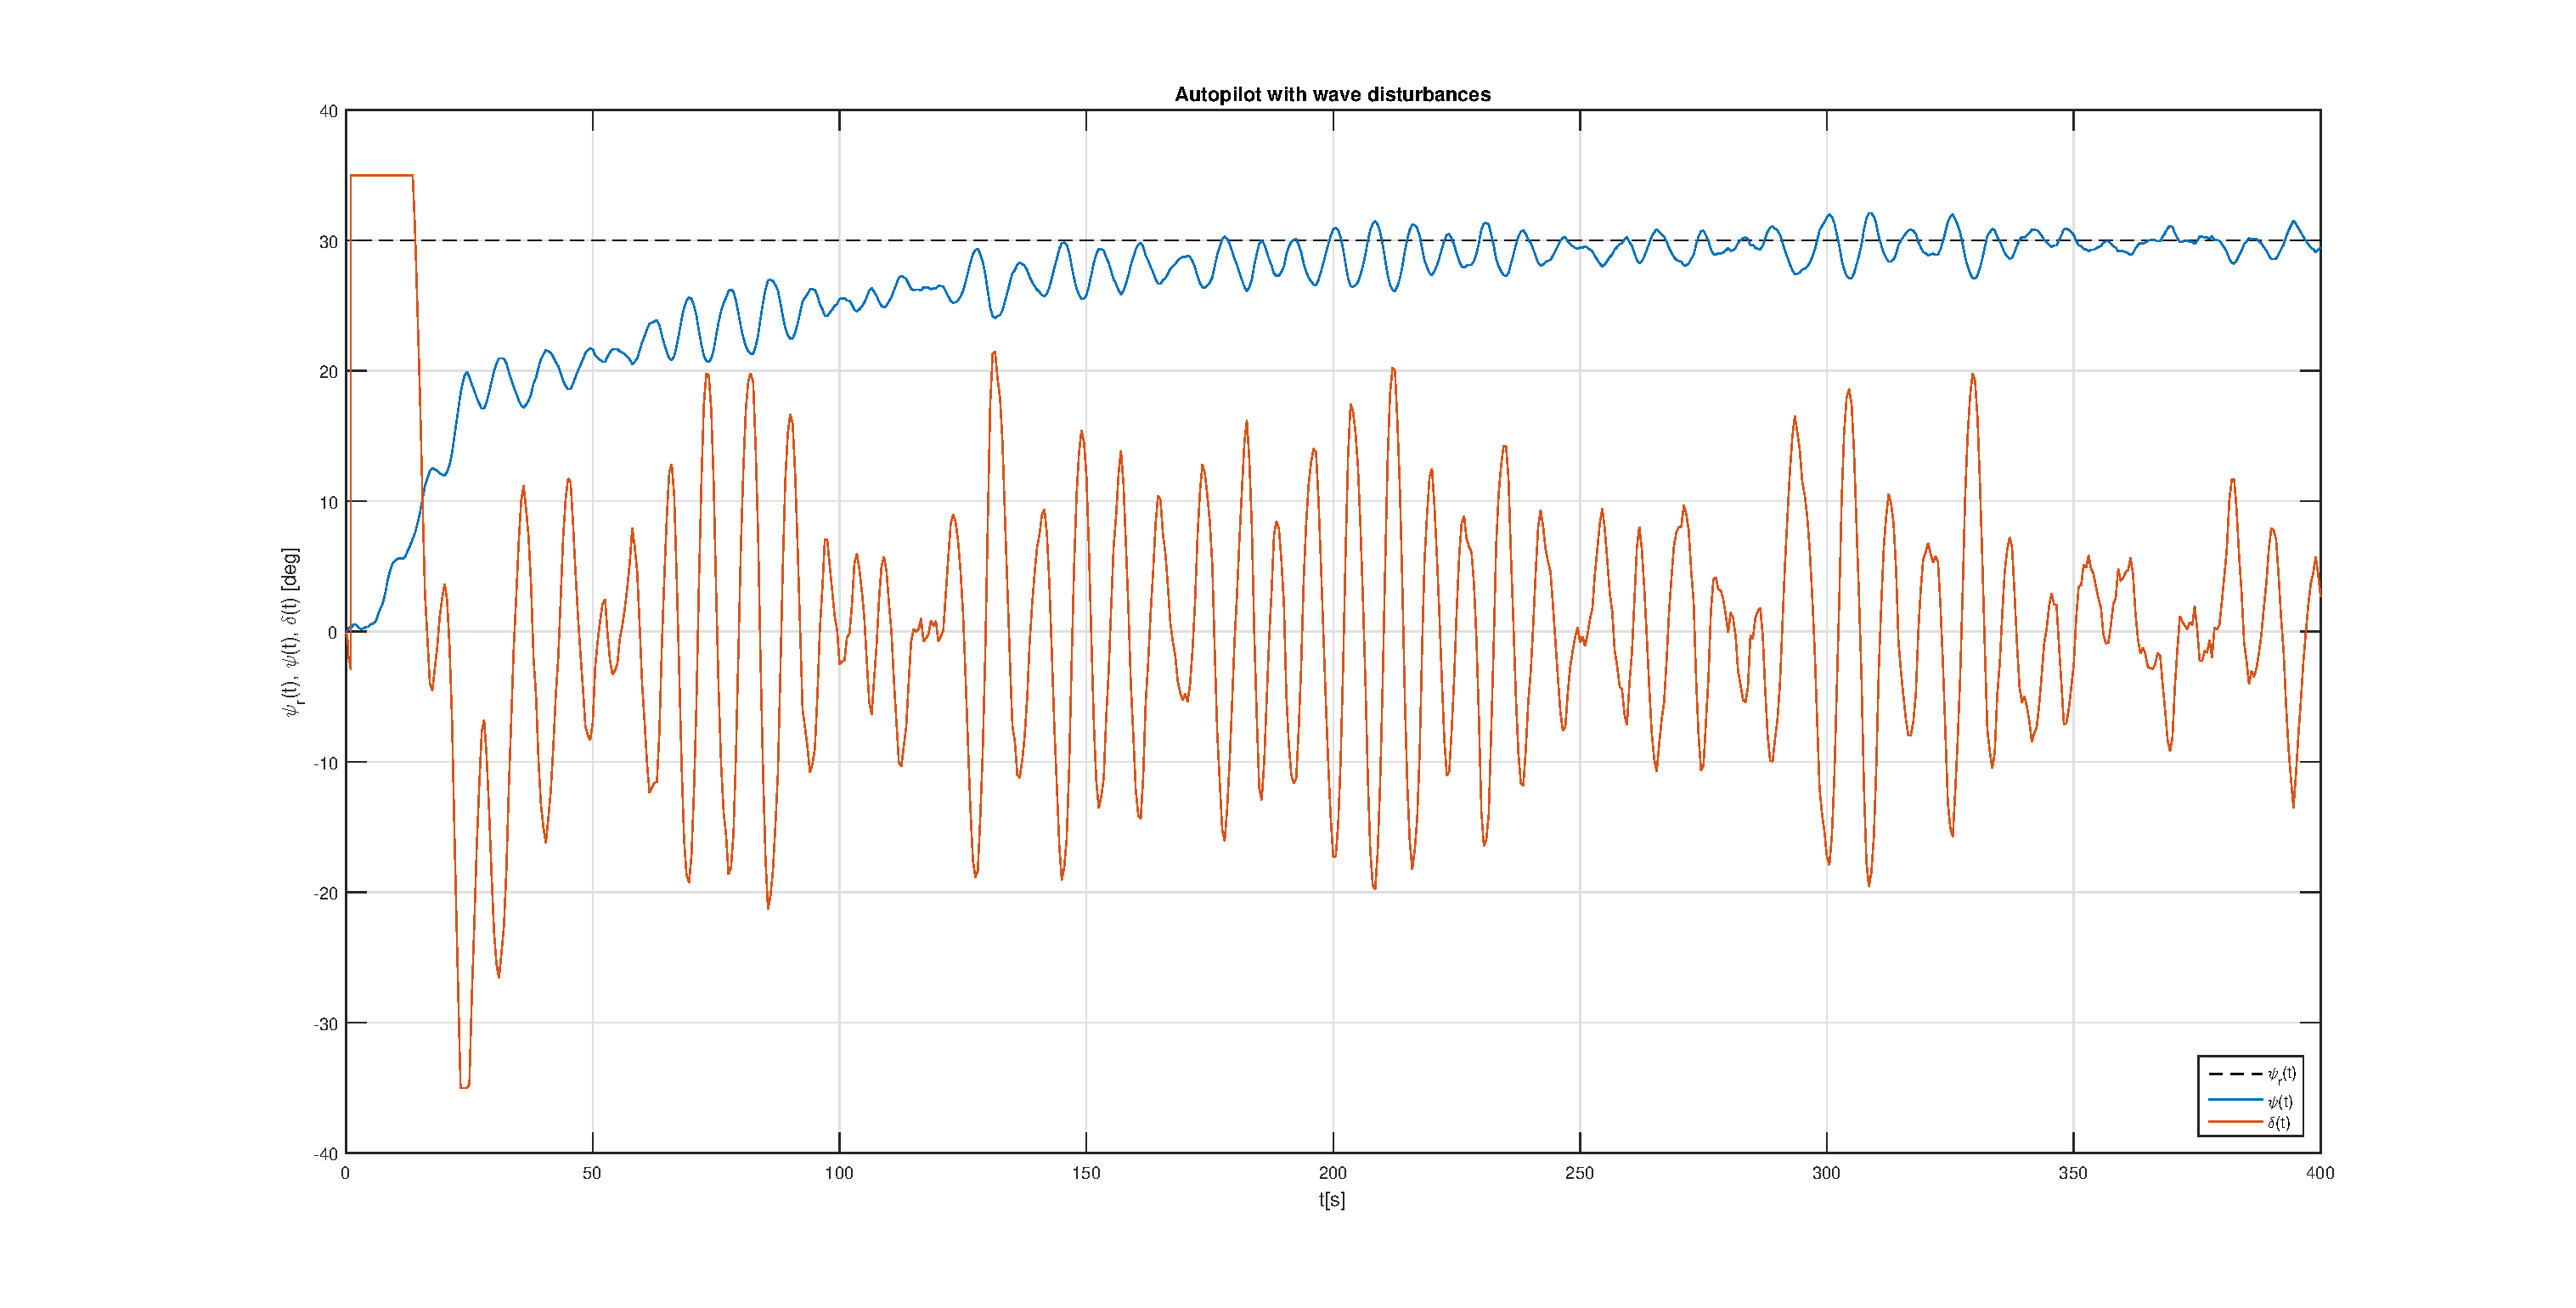
\includegraphics[scale=0.3]{plots/3d}} %This graph is simply too big, i'll fix later.
\label{plot:3d}
\end{figure}